\section{Arrays}

\textbf{Arrays Revisited}

As we have seen earlier, an array is a sequential collection of elements of a similar data type. In C\#, an array is an
object and thus a reference type, and therefore they are stored on the heap. We have only covered single dimension
arrays in the previous lessons, now we will explore multidimensional arrays.\\

\textbf{Multidimensional Arrays}\\

A multidimensional array is an ’array of arrays’. A multidimensional array is the one in which each element of the
array is an array itself. It is similar to tables in a database where each primary element (row) is a collection of
secondary elements (columns). If the secondary elements do not contain a collection of other elements, it is called
a 2-dimensional array (the most common type of multidimensional array), otherwise it is called an n-dimensional
array where n is the depth of the chain of arrays. There are two types of multidimensional arrays in C\#:

\begin{itemize}
    \item Rectangular array (one in which each row contains an equal number of columns)
    \item Jagged array (one in which each row does not necessarily contain an equal number of columns) 
\end{itemize}

The images below show what the different kinds of arrays look like. The figure also shows the indexes of different
elements of the arrays. Remember, the first element of an array is always zero (0).

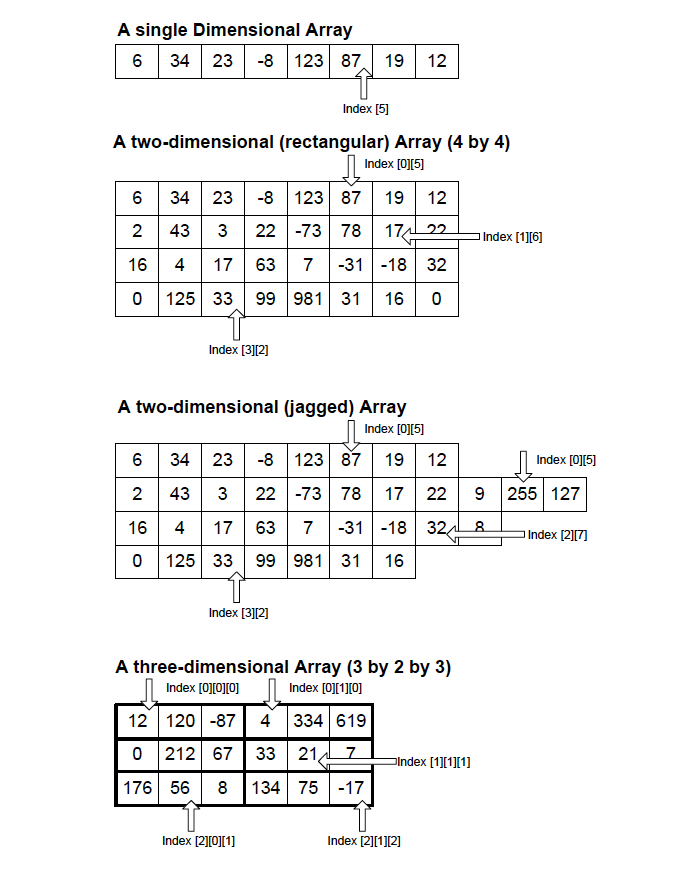
\includegraphics[width=1\linewidth]{Arrays.png}


\textbf{Instantiating and accessing the elements of multidimensional arrays}\\

Recall that we instantiate our single dimensional array like this:\\

\begin{lstlisting}
    int [] intArray = new int[5];    
\end{lstlisting}

The above line would instantiate (create) a one dimensional array (intArray) of type int, and with 5 elements. We
can access the elements of the array like this:\\

\begin{lstlisting}
    intArray[0] = 45; // set the first element to 45
    intArray[2] = 21; // set the third element to 21
    intArray[4] = 9; // set the fifth and last element to 9        
\end{lstlisting}

Instantiating a multidimensional array is almost identical to the above procedure, as long as you keep the most
basic definition of the multidimensional array in mind which says ’a multidimensional array is an array of arrays’.
Suppose we wish to create a two dimensional rectangular array with 2 rows and 3 columns. We can instantiate the
array as follows:

\begin{lstlisting}
    int [,] myTable = new int[2,3];    
\end{lstlisting}

All the elements of the array are auto-initialized to their default values; hence all the elements of the myTable array
would be initialized with zeroes. We can iterate through this array using either a foreach loop or a for loop.

\begin{lstlisting}
    foreach(int intVal in myTable)
    {
        Console.WriteLine(intVal);
    }        
\end{lstlisting}

When it is compiled and executed, it will print six (2 x 3) zeros.

\begin{lstlisting}
    0
    0
    0
    0
    0
    0        
\end{lstlisting}

Now, let us change the values of the individual elements of the array. To change the value of the first element of
the first row to 32, we can write the following code:

\begin{lstlisting}
    myTable[0,0] = 32;    
\end{lstlisting}

In the same way we can change the values of other elements of the array:

\begin{lstlisting}
    myTable[0,1] = 2;
    myTable[0,2] = 12;
    myTable[1,0] = 18;
    myTable[1,1] = 74;
    myTable[1,2] = -13;        
\end{lstlisting}

Now, we can use a couple of nested for loops to iterate over the array:

\begin{lstlisting}
    for(int row=0; row<myTable.GetLength(0); row++)
    {
        for(int col=0; col<myTable.GetLength(1); col++)
        {
            Console.WriteLine("Element at {0},{1} is {2}", row, col, myTable[row,col]);
        }
    }        
\end{lstlisting}

Here, we have used two for loops to iterate through each of the two dimensions of the array. We have used the
GetLength() method of the System.Array class (the underlying class for arrays in .Net) to find the length of a
particular dimension of an array. Note that the Length property will give total number of elements in this two
dimensional array, i.e., 6. The output of the above program will be:

\begin{lstlisting}
    Element at 0,0 is 3
    Element at 0,1 is 2
    Element at 0,2 is 12
    Element at 1,0 is 18
    Element at 1,1 is 74
    Element at 1,2 is -13        
\end{lstlisting}

\textbf{Instantiating and accessing Jagged Arrays}\\

A jagged array is one in which the length of each row is not the same. For example we may wish to create a table
with 3 rows where the length of the first row is 3, the second row is 5 and the third row is 2. We can instantiate this
jagged array like this:


\begin{lstlisting}
    int [][] myTable = new int[3][];
    myTable[0] = new int[3];
    myTable[1] = new int[5];
    myTable[2] = new int[2];        
\end{lstlisting}

Then we can fill the array like this:

\begin{lstlisting}
    myTable[0][0] = 3;
    myTable[0][1] = -2;
    myTable[0][2] = 16;
    myTable[1][0] = 1;
    myTable[1][1] = 9;
    myTable[1][2] = 5;
    myTable[1][3] = 6;
    myTable[1][4] = 98;
    myTable[2][0] = 19;
    myTable[2][1] = 6;        
\end{lstlisting}

Now, we will show how to use the foreach loop to access the elements of the array:

\begin{lstlisting}
    foreach(int []row in myTable)
    {
        foreach(int col in row)
        {
            Console.WriteLine(col);
        }
        Console.WriteLine();
    }        
\end{lstlisting}

The code above is very simple and easily understandable. We picked up each row (which is an int array) and then
iterated through the row while printing each of its columns. The output of the above code will be:


\begin{lstlisting}
    3
    -2
    16
    1
    9
    5
    6
    98
    19
    6        
\end{lstlisting}

In the same way, we can use a three-dimensional array:

\begin{lstlisting}
    int [,,] myTable = new int[3,2,4];
    myTable[0,0,0] = 3;
    myTable[1,1,1] = 6;        
\end{lstlisting}

Or in jagged array fashion:

\begin{lstlisting}
    int [][][] myTable = new int[2][][];
    myTable[0] = new int[2][];
    myTable[0][0] = new int[3];
    myTable[0][1] = new int[4];
    myTable[1] = new int[3][];
    myTable[1][0] = new int[2];
    myTable[1][1] = new int[4];
    myTable[1][2] = new int[3];
    myTable[0][0][0] = 34;
    myTable[0][1][1] = 43;
    myTable[1][2][2] = 76;        
\end{lstlisting}

Here, we have created a three dimensional jagged array. It is an array of two 2-dimensional arrays. The first of the
2-dimensional arrays contains 2 rows. The length of the first row is 3, while the length of second row is 4. In a
similar fashion, the second two dimensional array is also initialized. In the end, we have accessed some of the
elements of the array and assigned them different values. Although higher dimensional jagged arrays are quite
difficult to perceive; they may be very useful in certain complex problems. Again, the key to avoid confusion in
multidimensional arrays is to perceive them as an ’array of arrays’.\\

\textbf{Some other important points about multidimensional arrays}\\

In the examples we just saw, we have used multidimensional arrays of only the integer type. But, you can declare
arrays of any data type. For example, you may define an array of strings or even an array of objects of your own
class.

\begin{lstlisting}
    string []names = new string[4];    
\end{lstlisting}

You can initialize the elements of an array on the fly in the following ways

\begin{lstlisting}
    string []names = new string[4]{"Faraz", "Gates", "Hejlsberg", "Gosling"};    
\end{lstlisting}

or

\begin{lstlisting}
    string []names = new string[]{"Faraz", "Gates", "Hejlsberg", "Gosling"};    
\end{lstlisting}

or

\begin{lstlisting}
    string []names = {"Faraz", "Gates", "Hejlsberg", "Gosling"};
\end{lstlisting}

You can also separate the declaration and initialization of an array reference and the array:

\begin{lstlisting}
    string []names;
    names = new string[4]{"Faraz", "Gates", "Hejlsberg", "Gosling"};        
\end{lstlisting}

You can also initialize two-dimensional arrays on the fly (along with the declaration)

\begin{lstlisting}
    string [][]nameLists = {new string[]{"Sanfy", "In"},
                            new string[]{"Hejlsberg", "Gosling", "Bjarne"}};        
\end{lstlisting}

Some of the more important properties \& methods that can be applied on arrays are:

\begin{itemize}
    \item Length gives the number of elements in all dimensions of an array
    \item GetLength(int) gives the number of elements in a particular dimension of an array
    \item GetUpperBound() gives the upper bound of the specified dimension of an array
    \item GetLowerBound() gives the lower bound of the specified dimension of an array 
\end{itemize}


\textbf{The foreach Loop}\\

We have been using the foreach loop for quite a long time now. Let us see how it works and how can we enable our
class to be iterated over by the foreach loop. For this, we need to implement the IEnumerable interface which
contains only a single method, GetEnumerator(), that returns an object of type IEnumerator. The IEnumerator
interface contains one public property (Current) and two public methods MoveNext() and Reset(). The Current
property is declared in the IEnumerator interface as:

\begin{lstlisting}
    object Current { get; }    
\end{lstlisting}

It returns the current element of the collection which is of object data type. The MoveNext() method is declared as:

\begin{lstlisting}
    bool MoveNext();    
\end{lstlisting}

It advances the current selection to the next element of the collection and returns true if the advancement is
successful, and false if the collection has ended. When MoveNext() is called for the first time, it sets the selection
to the first element in the collection which means that the Current property is not valid until MoveNext() has been
executed for the first time.\\

Finally, the Reset() method is declared as

\begin{lstlisting}
    void Reset();    
\end{lstlisting}

This method resets the enumerator and sets it to the initial state. After reset, MoveNext() will again advance the
selection to the first element in the collection.

Now we will show how to make a class that can be iterated over using the foreach loop, by implementing the
IEnumerable and IEnumerator interfaces.

\begin{lstlisting}
    using System;
    using System.Collections;
    namespace CSharpSchool
    {
        class Test
        {
            static void Main()
            {
                MyList list = new MyList();
                foreach(string name in list)
                {
                    Console.WriteLine(name);
                }
            }
        }
        class MyList : IEnumerable
        {
            static string []names = {"Sanfy", "In", "Hejlsberg", "Gosling", "Bjarne"};
            public IEnumerator GetEnumerator()
            {
                return new MyEnumerator();
            }
            
            private class MyEnumerator : IEnumerator
            {
                int index = -1;
                public object Current
                {
                    get { return names[index]; }
                }
                public bool MoveNext()
                {
                    if(++index >= names.Length)
                        return false;
                    else
                        return true;
                }
                public void Reset()
                {
                    index = -1;
                }
            }
        }
    }    
\end{lstlisting}

Here we have declared a class called MyList which contains a private nested class named MyEnumerator. The
class MyEnumerator implements IEnumerator by providing the implementation of its public property and
methods. The class MyList implements the IEnumerable interface and returns an object of type MyEnumerator in
its GetEnumerator() method. The class MyList contains a static array of strings called names. The MyEnumerator
class iterates through this array. It uses the integer variable index to keep track of the current element of the
collection. The variable index is initialized with -1. Each time the MoveNext() method is called, it increments it by
1 and returns true or false, depending on whether collection’s final element has been reached. The Current property
returns the indexth element of the collection while the Reset() method resets the variable index to -1 again.
In the Test class we have instantiated the MyList class and iterated through it using a foreach loop, because we
have implemented IEnumerable interface on the MyList class. The output of the above program is:

\begin{lstlisting}
    Sanfy
    In
    Hejlsberg
    Gosling
    Bjarne    
\end{lstlisting}